% !TEX root = main.tex

\section{Constraint solving}

Constraint-satisfaction problems arise in many domains, including analysis, testing, and verification of software programs. Constraint solvers are decision procedures for problems expressed in logical formulas: for instance, the boolean satisfiability problem (also known as {\em SAT}) aims to determine whether there exists an interpretation of the symbols of a formula that makes it true. Although SAT is a NP-complete problem, recent advances have moved the boundaries for what is intractable when it comes to practical applications~\cite{SMT-CACM11}. 

Observe that some problems are more naturally described with languages that are more expressive than the one of boolean formulas with logical connectives. For this reason, satisfiability modulo theories (SMT) generalize the SAT problem with supporting theories to capture formulas involving, for instance, linear arithmetic inequalities and operations over arrays. SMT solvers map the atoms in an SMT formula to fresh boolean variables: a SAT decision procedure checks the rewritten formula for satisfiability, and a theory solver checks the model generated by the SAT procedure. We have informally discussed the theory of bit-vectors and arrays in Section \missing.

\mynote{Mention STP, Z3 and some others}However, despite the significant advances observed over the past few years -- which also made symbolic execution practical in the first place~\cite{CS-CACM13} -- constraint solving remains an important performance bottleneck in symbolic execution engines. Several optimizations have thus been developed in order to reduce both the number of invocations of the solver and the size of the formulas to check, so to avoid scalability problems arising when too large queries result in blowing the solver up. We discuss a number of such techniques in the remainder of this section.

%A significant amount of the execution time of a symbolic engine is spent invoking the constraint solver.

% ---------------------------------------------------------------------------------------------------
\subsection{Lazy evaluation}\mynote{citations?}
\mynote{[D] original text starts here} A technique used in practice to avoid frequent invocation of the constraint solver is {\em lazy evaluation}. The main idea is to avoid checking for contradictions at each branch condition, exploring both branches. This means that some of the states that the engine will later explore may be non-reachable during a real program execution. This allows a symbolic engine to quickly explore paths but forces it to check their consistency before using them for drawing some conclusions. The main disadvantages of this techniques are: (a) this strategy may lead to a large number of active states, (b) the time spent for checking the consistency of many states may be similar to the time spent for performing pruning in the first place.

% ---------------------------------------------------------------------------------------------------
\subsection{Solvers}
A list of constraint solvers\mynote{Table?}:
\begin{itemize}
  \item \cite{STP-TR07}: used by~\cite{EXE-CCS06,KLEE-OSDI08,MineSweeper-BOTNET08}, used by SPF
  \item \cite{Z3-TACS08}: used by~\cite{FIRMALICE-NDSS15,MAYHEM-SP12}
  \item \cite{DISSOLVER-TR03}: initially used by \cite{SAGE-NDSS08}
  \item \cite{PPL-SCP08}: used by \cite{AEG-NDSS11}
  \item (incremental solver) \href{http://www.cs.nyu.edu/acsys/cvc3/}{CVC3}: an automatic theorem prover for Satisfiability Modulo Theories, used by SPF
  \item (incremental solver) \href{http://yices.csl.sri.com/}{Yices}: The Yices SMT Solver~\cite{YICES-CAV06}
  \item \href{http://choco-solver.org/}{CHOCO}: A Free and Open-Source Java Library for Constraint Programming, used by SPF
  \item \href{http://www.cs.brandeis.edu/~tim/Applets/IAsolver.html}{IAsolver}: the Brandeis Interval Arithmetic Constraint Solver, used by SPF
  \item \href{https://people.csail.mit.edu/akiezun/hampi/}{Hampi}: A Solver for String Constraints, used by SPF
  \item \href{https://www.cs.umd.edu/projects/omega/}{Omega}~\cite{OMEGA-SC91}, used by SPF
  \item \href{http://pagesperso.lina.univ-nantes.fr/~granvilliers-l/realpaver/}{RealPaver}: onlinear constraint solving \& rigorous global optimization, used by SPF
  \item \href{http://smtlib.cs.uiowa.edu/}{SMT-LIB}: the satisfiability modulo theories library, used by SPF
  \item CORAL~\cite{CORAL-NFM11}: used by SPF
\end{itemize}

% ---------------------------------------------------------------------------------------------------
\subsection{Dealing with unsolvable constraints} 

Assume to start a concrete execution with a concrete input and in parallel symbolically execute the same program. Whenever a set of constraints cannot be solved by the constraint solver, then use the concrete value to proceed into at least one branch. Example taken from~\cite{CS-CACM13}:
    \begin{lstlisting}[basicstyle=\ttfamily\small]
    int non_linear(int v) {
      return (v * v) % 50;
    }
    \end{lstlisting}
The non-linear operation inside this function can be hard for a solver. Using a concrete execution, the engine can overcome this problem, but then the precision and completeness may be affected.

Notice that the use of concrete values can also avoid to perform alias analysis on pointers, which is typically very expensive. Whenever meaningful, \cite{DART-PLDI05} tries to test both valid (not {\tt NULL}) and invalid ({\tt NULL}) input pointers in order to maximize bug detection. However~\cite{DART-PLDI05} will never artificially negate a branch if that condition cannot be exercised using a concrete input. In other words, both branches of an {\tt if} statement are considered only if they are both meaningful (more precisely: \cite{DART-PLDI05} is able to generate a valid input). Notice that~\cite{DART-PLDI05} may generate an input using a solver by considering only a subset of branch constraints. For instance, consider constraints ($C_1, C_2, C_3$) given by three nested branches: if $C_1$ is non linear (hard to solve), it needs only to generate a random input for taking $C_1$ and then use the solver for exploring path given by $(C_2, C_3)$. A traditional symbolic execution engine may get stuck at $C_1$ and give up after some time on {\em all} the derived path. Notice that whenever a concrete input is used to overcome a hard constraint, the overall approach become incomplete.

% ---------------------------------------------------------------------------------------------------
\subsection{Constraint optimizations}
\label{constraint-optimizations}

\mynote{add \cite{S-FMCAD08} + some optimizations listed in Section~\ref{memory-model}.}

Many optimization can be applied to constraints in order to make it more solver-friendly.

\subsubsection{Constraint caching} Cache solver results and reuse them \mynote{to be completed}

\subsubsection{Constraint independence} tracks constraints into multiple independent subsets of constraints, This helps the system discards irrelevant constraints and adds additional cache hits.  \mynote{to be completed}

\subsubsection{Irrelevant constraint optimization} Remove from path constraints those constraints that are irrelevant in deciding the outcome of the current branch. In practice, this is done by computing the transitive closure of all the constraints. Pointer and array reference can make this hard: e.g., see details in~\cite{EXE-CCS06,EGL-ISSTA09,CUTE-FSE13}. In~\cite{KLEE-OSDI08}, this is called {\em constraint independence}: the main idea is to divide constraints in independent disjoint subsets based on the symbolic variables which they reference. Irrelevant constraints can detected and discarded.

\subsubsection{Incremental solving} Many paths common branches, then it can be beneficial to reason about subset or superset of constraints. See more details, e.g., in~\cite{KLEE-OSDI08,CUTE-FSE13}. In~\cite{KLEE-OSDI08}, they propose {\em counterexample caching} to keep a cache of counterexample based on past queries:
      \begin{itemize}
        \item if a subset of constraints has not solution, any superset does not have as well
        \item if a superset has a solution, any subset has a solution
        \item if a subset has a solution, try it for the superset
      \end{itemize}

\subsubsection{Bit-field theory expression} \cite{CKC-TOCS12} tries to simplify expression using a bit-field theory expressions: if parts of a symbolic variable are masked away by bit operations, then known bits of the symbolic variable can be replaced by their constant values. If all bits of a symbolic variable are constant, then the variable is marked as concrete.

\subsubsection{Page boundings on pointers} Whenever a memory access with a symbolic pointer occurs,~\cite{CKC-TOCS12} determines the page referenced by the pointer. This information is then passed to the solver to help it. To make this even more effective, the page size is reduced as much as possible (e.g., 128 bytes).

%{\em Concolic execution} has been originally introduced in~\cite{DART-PLDI05} and then refined by~\cite{CUTE-FSE13}. A common disadvantage of symbolic execution is that the state space can be exponential. Moreover, even when the state space is tractable it may happen that complex constraints need to be solved but these constraints are too complex for the actual solver (e.g., non-linear constraints are typically hard to solve). For this reason, it is common to exploit concolic execution. 

\subsubsection{Generational Search}
%{\em Use concolic execution to generate useful (random) inputs.} 
Starts concrete execution using a random (concrete) input and for each taken branch tracks the input constraints by observing the branch condition. When the execution is completed, restart another concrete execution using a different concrete random input that is compliant with the constraints but explore a new path. It is sufficient to negate a single constraint given by a conditional branch, to explore a different path. Keep track of taken branches with binary values. An algorithm for maximizing coverage is proposed in~\cite{DART-PLDI05}. Notice that the symbolic execution is performed in parallel with the concrete execution. Related examples are~\cite{SAGE-NDSS08,DRILLER-NDSS16}. \mynote{Add paper on hybrid concolic testing}In particular,~\cite{DRILLER-NDSS16} is an example of {\em symbolic-assisted fuzzing}: their technique temporarily exploits concolic execution only when a fuzzer cannot generate a valid input to explore an uncovered branch.

\paragraph{An example}\mynote{Improve this discussion} Given a concrete input, an application will execute only a subsets of its basic blocks $B_i$. Moreover, they will be executed following a specific order. For instance, the program execution shown in Figure~\ref{fig:example-concrete-execution}a has executed the sequence of basic blocks $\{B_1, B_2, B_4, B_6\}$. Other blocks, such as $B_3$, have not been executed due to non-taken branches. Driven by the concrete execution, a symbolic execution engine may trace symbolic constraints on the taken branches and then generate an input that forces the execution to take a never-taken branch. For instance, if the symbolic execution engine may want to generate an input that executes basic block $B_5$, then it traces the constraints on the two taken branches and then negate the constraint on the branch that leads the execution toward $B_5$. Figure~\ref{fig:example-concrete-execution}b provides the logical steps performed by the engine.

\begin{figure}[t]
  \vspace{-3mm}
  \centering
  \begin{subfigure}{.5\textwidth}
    \centering
    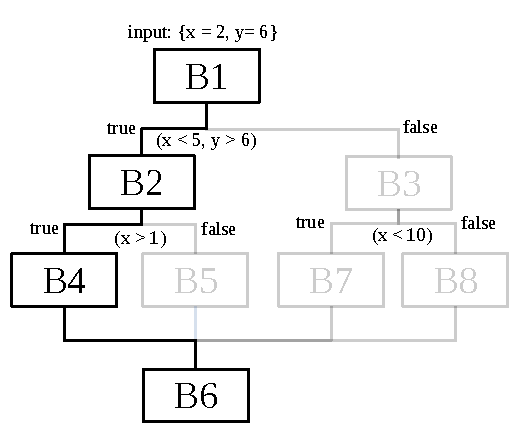
\includegraphics[width=0.9\columnwidth]{images/concrete-execution} 
    %\label{fig:sub1}
    \vspace{15mm}
    \caption{}
  \end{subfigure}%
  \begin{subfigure}{.5\textwidth}
    \centering
    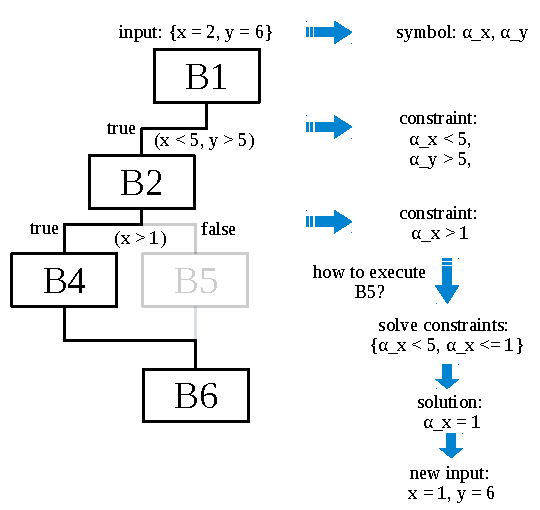
\includegraphics[width=1.0\columnwidth]{images/concolic-execution} 
    %\label{fig:sub2}
    \caption{}
  \end{subfigure}
  \caption{(a) a concrete execution of a program. Only a subset of basic blocks is executed. The sequence of executed basic blocks is $\{B_1, B_2, B_4, B_6\}$. (b) concolic execution for generating an input that executes $B_5$.}
  \label{fig:example-concrete-execution}
  \vspace{-3mm}
\end{figure}

\subsubsection{Execution-Generated Testing (EGT)} 
Is the approach used by some papers (e.g.,~\cite{KLEE-OSDI08,EXE-CCS06}) that works by making a distinction between the concrete and symbolic state of a program: if an operation involves only concrete values, then the symbolic engine concretely execute it. This can allow symbolic execution to reason even over complex operation (e.g., non linear operations) if they involve only concrete values. EGT is often seen (\cite{CS-CACM13}) as a form of dynamic symbolic execution: this can be seen as more general term than concolic execution.